\input{../head.tex}

\section{Approximation de la fréquence de coupure}

Cette section a pour but d'expliquer notre démarche pour l'approximation de la fréquence de coupure
dans un circuit passe-bas et passe-haut. Trois méthodes nous étaient proposées, et nous avons adopté
la première pour les raisons explicitées plus bas.

Définissons tout d'abord ce qu'est la fréquence de coupure. Dans le cas d'un filtre passe-bas, toutes les fréquences qui
lui sont supérieures ne passent pas et, inversément, pour un passe-haut seules les fréquences supérieures passent.
En terme de tension, dans le premier cas, la tension de sortie reste constante jusqu'à qu'à la fréquence de coupure,
à partir de laquelle elle diminue exponentionnellement. Inversément, pour un filtre CR, la tension croît
exponentiellement avant de se stabiliser après la fréquence de coupure.

Pour la déterminer, nous avons tout d'abord procédé à une expérience en laboratoire.
Celle-ci consistait à mesurer la tension de sortie en fonction de la fréquence du signal, et ce dans
chacun des circuits considérés. Nous ne vous présenterons ici que la démarche pour le filtre passe-bas, 
la méthode étant similaire pour le passe-haut.
Graphiquement, le tracé du rapport des tensions d'entrée et de sortie des filtres en fonction de la
fréquence a l'allure d'une exponentielle. Pour faciliter le calcul, nous sommes passés en repère
semi-logarithmique, réduisant ainsi l'exponentielle à une intersection de deux droites. Ce procédé est
explicité en profondeur dans la sous-section "Passage en échelle logarithmique"'.

\subsection{Filtre passe-bas}

\begin{figure}[ht!]
\centering
\begin{tikzpicture}
\begin{axis}[
xlabel={$\log f$},
ylabel={$V_{out}$},]
\addplot coordinates
{(0,2.5) (5000,2.5) (10000,2.5) (16000,1.7) (18000,1.55) (20000,1.45)};
\end{axis}
\end{tikzpicture}
\caption{Graphe de $V_{out}$ expérimentale en fonction de la fréquence}
\label{lwp_ratio}
\end{figure}

\paragraph{Équation de la droite horizontale}
Expérimentalement, nous obtenons une fréquence de sortie constante (de $\unit{2.5}{\volt}$ )
pour les plus basses fréquences. L'équation de la droite horizontale est donc :

$$y=2.5$$

\paragraph{Équation de la droite diagonale}

Avec les mesures effectuées en laboratoire, nous n'obtenons non pas une droite mais bien une exponentielle.
Pour faciliter le calcul de l'intersection de l'exponentielle et de la droite, nous passons donc en repère
semi-logarithmique.

Nous savons que l'équation d'une droite dans un repère cartésien est de type $y=ax+b$, avec $a$ la pente
et $b$ l'ordonnée à l'origine.

Mais ici nous ne sommes plus dans un repère cartésien mais bien dans un répère semi-log selon l'axe des
abscisses. L'équation de la droite devient alors : $y=a\log{x}+b$.

\paragraph{Mesures en laboratoire}

Voici 3 résultats choisis de manière cohérente parmi toutes les mesures effectuées en laboratoire, où
$V_c$ est la tension de sortie et $f$ la fréquence :

\begin{center}
\begin{tabular}{|c|c|c|}
\hline
$V_c$ & $f$ & $\log{f}$ \\
\hline
1.7 & 16000 & 4.204 \\
\hline
1.55 & 18000 & 4.255 \\
\hline
1.45 & 20000 & 4.301 \\
\hline
\end{tabular}
\end{center}

Dès maintenant, les fréquences sont exprimées en base logarithmique.
Écrivons un système ayant pour inconnues la pente ($a$) et l'ordonnée à l'origine ($b$) de notre droite
inconnue.
Nous avons trois équations à deux inconnues, et le système n'admet pas de solution.
Cela n'est pas étonnant, étant donné que les résultats expérimentaux ne sont jamais très précis.

Voici le système sous forme matricielle :

$$A \cdot \vec{x} = \vec{b}$$

$$
\begin{pmatrix}
4.204 & 1\\
4.255 & 1 \\
4.301 & 1
\end{pmatrix} 
\begin{pmatrix}
a\\
b
\end{pmatrix} 
= 
\begin{pmatrix}
1.7\\
1.55\\
1.45
\end{pmatrix}
$$
	

Le système n'admet pas de solution car $\vec{b}$ n'appartient pas à l'espace des colonnes de $A$. Nous
allons donc projeter $\vec{b}$ sur l'espace des colonnes de $A$ afin d'obtenir une solution approchée.

Soient $f_1$, $f_2$ les colonnes de $A$, et donc les éléments de la base de l'espace des colonnes de $A$.
Trouvons une base orthonormée $(e_1, e_2)$ de l'espace colonnes de la matrice en utilisant
la méthode de \textsc{Gram-Schmidt}:

$$ \vec {e_1} = \frac{f_1}{||f_1||} = \begin{pmatrix} \frac{1}{\sqrt{3}} & \frac{1}{\sqrt{3}} &\frac{1}{\sqrt{3}}) \end{pmatrix}$$

$$ \vec {e_2} = \frac{ \vec{f_2} - (\vec{e_1}|\vec{f_2})}{||\vec{f_2} - (\vec{e_1}|\vec{f_2})||} = \begin{pmatrix}
-0.684 & 0.03 & 0.729 \end{pmatrix} $$

Nous sommes maintenant en mesure de trouver une projection du vecteur contenant nos données expérimentales
peu précises :
nous projetons les vecteurs grâce à la formule de la projection :

% Peut-être parler ici du fait qu'on projete plutôt sur A orthogonal pour gagner du temps en calcul ?

$$
\vec{b'}
=
(\vec{b}|\vec{e_1}) \cdot \vec{e_1} + (\vec{b}|\vec{e_2}) \cdot \vec{e_2}
=
\begin{pmatrix}
1.607\\
1.556\\
1.524
\end{pmatrix}
$$

Nous pouvons alors réécrire le système comme cela :

$$
\begin{pmatrix}
 4.204 & 1\\
 4.255 & 1 \\
 4.301 & 1
\end{pmatrix}
\begin{pmatrix}
a\\
b
\end{pmatrix}
=
\begin{pmatrix}
1.607\\
1.565\\
1.524
\end{pmatrix}
$$

Nous en déduisons la valeur des coefficients $a$ et $b$ :

$$a = -1.96$$
$$b= 9.84$$

La droite oblique a donc pour équation
$$y= -1.96 \log x + 9.84$$

Pour trouver la fréquence d'intersection entre les deux droites, nous résolvons le système, et nous
trouvons :

$$x = \unit{5557.7}{\hertz}$$

Cela nous semble correct car en théorie nous devions arriver à une valeur $f$ telle que :

$$f=\frac{1}{2\pi RC}$$

avec $R= 7.5 + 50 = \unit{57.5}{\ohm}$ \footnote{\unit{50}{\ohm} est la résistance interne du générateur de signaux utilisé
en laboratoire pour l'expérience et \unit{7.5}{\ohm} est la résistance utilisée pour constituer le filtre.} et 
$C= \unit{470 \cdot 10^{-9}}{\farad}$, la valeur théorique de la fréquence de coupure est donc :

$$f= \unit{5889.2}{\hertz}$$

Afin de visualiser l'approximation que nous avons effectuée, il est intéressant de comparer la courbe 
théorique avec les deux droites obtenues. Sur la Figure \ref{label}, nous remarquons que les fréquences
de coupure se superposent, tellement elles sont proches l'une de l'autre.

\begin{figure}[!htb]
	\centering
	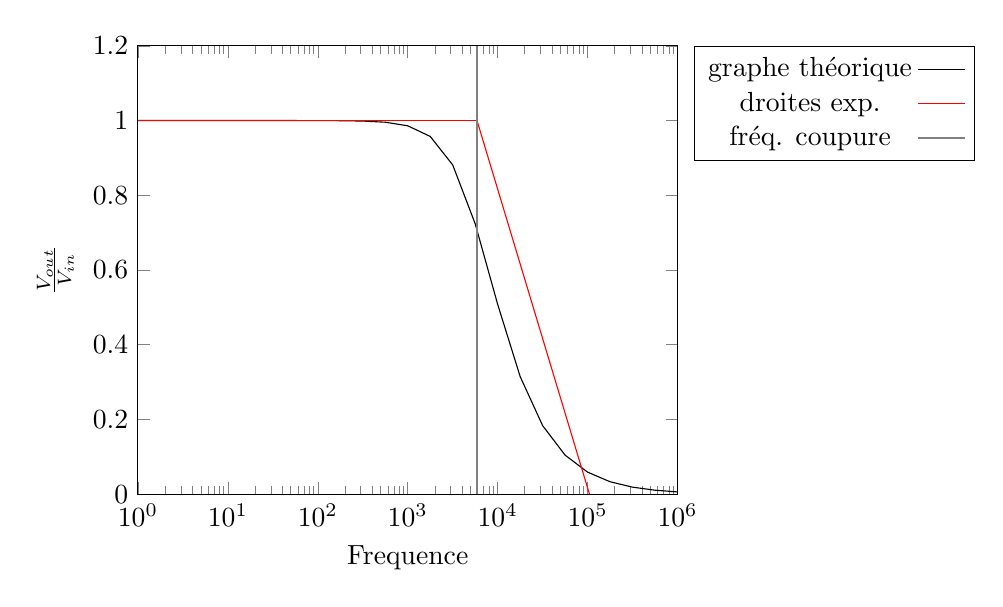
\begin{tikzpicture}[>=stealth]
\begin{semilogxaxis}[legend entries = {graphe théorique, droites exp., , fréq. coupure},legend style={at={(1.03,1)}, anchor=north west}, legend plot pos=right, xlabel=Frequence, ylabel= $\frac{V_{out}}{V_{in}}$, xmin=1, xmax=1000000, ymin=0, ymax=1.2]

\addplot[domain=1:1e6, black] {(1/((1 + (2*3.14*x*57.5*0.00000047)^2)^(0.5))};
\addplot[no marks, red] coordinates
{(1,1) (5889,1)};
\addplot[no marks, red] coordinates
{(5889,1) (104811,0)};
\addplot[no marks, gray] coordinates
{(5889,0) (5889,1.2)};

\end{semilogxaxis}
	\end{tikzpicture}
	\label{label}
	\caption{Confrontation du graphe théorique et des droites expérimentales}
\end{figure}

\subsection{Choix de la méthode}

Une démarche d'approximation n'est évidemment pas unique. Nous avions le choix entre trois méthodes
distinctes, et nous avons opté pour celle utilisant les bases orthonormées.

Les trois méthodes proposées suivaient la même démarche : minimiser une distance afin de déterminer une droite. 

Pour la première méthode, nous devions minimiser la distance entre un polynôme de degré \numprint{2} passant par nos
points mesurés au laboratoire et la droite à déterminer :

Soit la droite à déterminer $H(x) = ax + b$ et le polynôme $q(x) = \alpha x^2 + \beta x + \gamma$, nous
cherchons à déterminer la distance :

$$\dist({H-q})^2 = (H-q|H-q) = (H(x_1)-q(x_1))^2 + (H(x_2)-q(x_2))^2 + (H(x_3)-q(x_3))^2$$

Sachant que $q(x_i) = y_i$, nous arrivons finalement :

$$\dist({H-q})^2 = (ax_1 + b - y_1)^2 + (ax_2 + b - y_2)^2 + (ax_3 + b - y_3)^2$$

Nous arrivons exactement à la même solution pour la seconde méthode qui minimise la fonction distance. 

Pour la troisième méthode, nous avons calculé la projection orthogonale de la colonne $y$ sur l'espace
des colonnes de la matrice de notre système. Cela revient à minimiser la distance entre le vecteur $y$ 
et la projection $y'$ :

$$\dist({y'-y})^2 = (y'-y|y'-y)$$

Nous savons que $y'_i = ax_1 + b$, nous pouvons donc dire que :

$$\dist({ax_1 + b - y_1})^2 + (ax_2 + b - y_2)^2 + (ax_3 + b - y_3)^2$$

Ce qui nous redonne la même solution que les deux autres méthodes. 
Néanmoins, les différents arrondis durant les calculs ont mené à des réponses sensiblement différentes. 
Pour cette raison, nous avons gardé la troisième méthode qui nous donne une fréquence de coupure la plus
proche de la fréquence théorique du filtre passe-bas.
 
\subsection{Meilleure approximation}
Pour arriver à une meilleure approximation, nous pourrions imaginer considérer $n$ points avec un
$n$ très grand. Cependant, déterminer l'unique polynôme de degré $n-1$ passant par les trois points 
serait assez vite difficile à déterminer. Le produit scalaire défini étant dépendant 
des $n$ points, résoudre ce problème sans logiciel devient impossible quand $n$ est grand.  

\subsection{Passage en échelle logarithmique}
Lors de notre approximation, nous avons mentionné le fait que nous "passions en échelle logarithmique".
Généralement, nous utilisons des échelles linéaires, avec des graduations dont la différence est constante.
Ici, dans un souci de facilité, nous avons utilisé une représentation semi-logarithmique. Cela signifie
que les graduations ont un rapport constant, et non plus une différence constante pour l'axe des abscisses.
Cela nous permet de travailler à grande échelle, et de représenter l'exponentielle comme une droite, de
manière simple. L'équation de la droite horizontale devient, en toute généralité : $y=a\log{x}+b$ .

\input{../foot.tex}
